\documentclass[xcolor=svgnames]{beamer}\usepackage{graphicx, color}
%% maxwidth is the original width if it is less than linewidth
%% otherwise use linewidth (to make sure the graphics do not exceed the margin)
\makeatletter
\def\maxwidth{ %
  \ifdim\Gin@nat@width>\linewidth
    \linewidth
  \else
    \Gin@nat@width
  \fi
}
\makeatother

\definecolor{fgcolor}{rgb}{0.2, 0.2, 0.2}
\newcommand{\hlnumber}[1]{\textcolor[rgb]{0,0,0}{#1}}%
\newcommand{\hlfunctioncall}[1]{\textcolor[rgb]{0.501960784313725,0,0.329411764705882}{\textbf{#1}}}%
\newcommand{\hlstring}[1]{\textcolor[rgb]{0.6,0.6,1}{#1}}%
\newcommand{\hlkeyword}[1]{\textcolor[rgb]{0,0,0}{\textbf{#1}}}%
\newcommand{\hlargument}[1]{\textcolor[rgb]{0.690196078431373,0.250980392156863,0.0196078431372549}{#1}}%
\newcommand{\hlcomment}[1]{\textcolor[rgb]{0.180392156862745,0.6,0.341176470588235}{#1}}%
\newcommand{\hlroxygencomment}[1]{\textcolor[rgb]{0.43921568627451,0.47843137254902,0.701960784313725}{#1}}%
\newcommand{\hlformalargs}[1]{\textcolor[rgb]{0.690196078431373,0.250980392156863,0.0196078431372549}{#1}}%
\newcommand{\hleqformalargs}[1]{\textcolor[rgb]{0.690196078431373,0.250980392156863,0.0196078431372549}{#1}}%
\newcommand{\hlassignement}[1]{\textcolor[rgb]{0,0,0}{\textbf{#1}}}%
\newcommand{\hlpackage}[1]{\textcolor[rgb]{0.588235294117647,0.709803921568627,0.145098039215686}{#1}}%
\newcommand{\hlslot}[1]{\textit{#1}}%
\newcommand{\hlsymbol}[1]{\textcolor[rgb]{0,0,0}{#1}}%
\newcommand{\hlprompt}[1]{\textcolor[rgb]{0.2,0.2,0.2}{#1}}%

\usepackage{framed}
\makeatletter
\newenvironment{kframe}{%
 \def\at@end@of@kframe{}%
 \ifinner\ifhmode%
  \def\at@end@of@kframe{\end{minipage}}%
  \begin{minipage}{\columnwidth}%
 \fi\fi%
 \def\FrameCommand##1{\hskip\@totalleftmargin \hskip-\fboxsep
 \colorbox{shadecolor}{##1}\hskip-\fboxsep
     % There is no \\@totalrightmargin, so:
     \hskip-\linewidth \hskip-\@totalleftmargin \hskip\columnwidth}%
 \MakeFramed {\advance\hsize-\width
   \@totalleftmargin\z@ \linewidth\hsize
   \@setminipage}}%
 {\par\unskip\endMakeFramed%
 \at@end@of@kframe}
\makeatother

\definecolor{shadecolor}{rgb}{.97, .97, .97}
\definecolor{messagecolor}{rgb}{0, 0, 0}
\definecolor{warningcolor}{rgb}{1, 0, 1}
\definecolor{errorcolor}{rgb}{1, 0, 0}
\newenvironment{knitrout}{}{} % an empty environment to be redefined in TeX

\usepackage{alltt}
\usetheme{Boadilla}
\usecolortheme[named=SeaGreen]{structure}
\usepackage{graphicx}
\usepackage{breqn}
\usepackage{xcolor}
\usepackage{booktabs}
\usepackage{verbatim}
\usepackage{tikz}
\usetikzlibrary{shadows,arrows,positioning}
\definecolor{links}{HTML}{2A1B81}
\hypersetup{colorlinks,linkcolor=links,urlcolor=links}
\usepackage{pgfpages}

\tikzstyle{block} = [rectangle, draw, text width=9em, text centered, rounded corners, minimum height=3em, minimum width=7em, top color = white, bottom color=brown!30,  drop shadow]

\newcommand{\ShowSexpr}[1]{\texttt{{\char`\\}Sexpr\{#1\}}}
\IfFileExists{upquote.sty}{\usepackage{upquote}}{}

\begin{document}

\title[R with Microsoft]{A simple workflow for using R with Microsoft products}
\author[M. Beck]{Marcus W. Beck}

\institute[USEPA NHEERL]{USEPA NHEERL Gulf Ecology Division, Gulf Breeze, FL\\
Email: \href{mailto:beck.marcus@epa.gov}{beck.marcus@epa.gov}, Phone: 850 934 2480}

\date{May 21, 2014}

%%%%%%
\begin{frame}
\vspace{-0.3in}
\titlepage
\end{frame}

%%%%%%
\begin{frame}{The problem...}
\begin{itemize}
\item R is great and has an increasing user base\\~\\
\item RStudio is integrated with multiple document preparation systems \\~\\
\item Output documents are not in a format that facilitates collaboration with 
non R users, e.g., pdf, html \\~\\
\item Data coming to you may be in a proprietary format, e.g., xls spreadsheet
\end{itemize}
\end{frame}

%%%%%%
\begin{frame}{The solution?}
\begin{itemize}
\item Solution one - Make liberal use of `projects' within RStudio \\~\\
\item Solution two - Use \texttt{gdata} package to import excel data \\~\\
\item Solution three - Get pandoc to convert document formats - \href{http://johnmacfarlane.net/pandoc/}{http://johnmacfarlane.net/pandoc/} \\~\\
\end{itemize}
\onslide<2->
\large
\centerline{\textit{Not recommended for simple tasks unless you really, really love R}}
\end{frame}

%%%%%
\begin{frame}{An example workflow}
\begin{itemize}
\item I will present a workflow for integrating Microsoft products within RStudio as an approach to working with non R users \\~\\
\item Idea is to never leave the RStudio environment - dynamic documents! \\~\\
\item General workflow... \\~\\
\end{itemize}
\small
\begin{center}
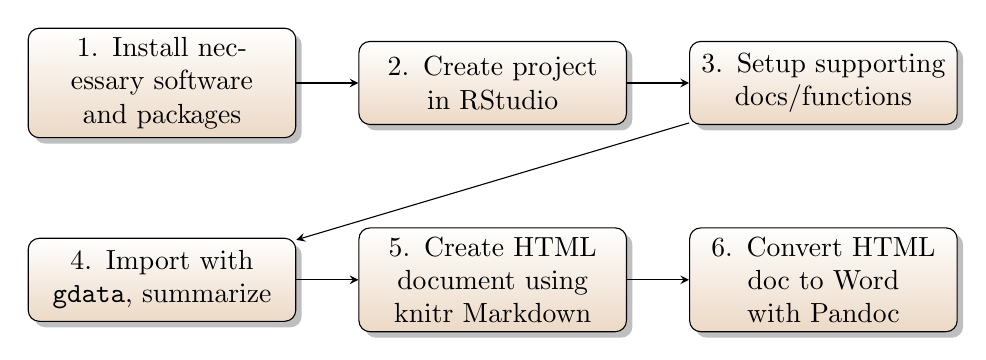
\begin{tikzpicture}[node distance=2.5cm, auto, >=stealth]
  \onslide<2->{
	\node[block] (a) {1. Install necessary software and packages};}
	\onslide<3->{
	\node[block] (b)  [right of=a, node distance=4.2cm] {2. Create project in RStudio};
 	\draw[->] (a) -- (b);}
 	\onslide<4->{
 	\node[block] (c)  [right of=b, node distance=4.2cm]  {3. Setup supporting docs/functions};
 	\draw[->] (b) -- (c);}
   \onslide<5->{
   \node[block] (d)  [below of=a, node distance=2.5cm]  {4. Import with \texttt{gdata}, summarize};
 	\draw[->] (c) -- (d);}
   \onslide<6->{
   \node[block] (e)  [right of=d, node distance=4.2cm]  {5. Create HTML document using knitr Markdown};
 	\draw[->] (d) -- (e);}
     \onslide<7->{
   \node[block] (f)  [right of=e, node distance=4.2cm]  {6. Convert HTML doc to Word with Pandoc};
   \draw[->] (e) -- (f);}
\end{tikzpicture}
\end{center}
\end{frame}

%%%%%%
\begin{frame}[shrink]{The example}
You are sent an Excel file of data to summarize and report but you love R and want to do everything in RStudio...
% latex table generated in R 3.1.0 by xtable 1.7-1 package
% Mon May 19 16:44:31 2014
\begin{table}[ht]
\centering
{\scriptsize
\begin{tabular}{lrrrlrr}
  \hline
SiteName & Year & Restoration & Reference & Observer.Names & Precipitation & Temperature \\ 
  \hline
IGH &  2005 &     3 &     3 & Tyler\_Amanda &     0 &    48 \\ 
  Kelly &  2005 &     4 &     2 & Patrick\_Chelsea &     0 &    48 \\ 
  Carlton &  2005 &     2 &     3 & David\_Megan &     0 &    48 \\ 
  IGH &  2006 &     9 &     6 & Tyler\_Amanda &     0 &    52 \\ 
  Kelly &  2006 &     9 &     1 & David\_Megan &     0 &    52 \\ 
  Carlton &  2006 &     7 &     3 & Patrick\_Chelsea &     0 &    52 \\ 
  IGH &  2007 &    12 &     7 & David\_Megan &    12 &    41 \\ 
  Kelly &  2007 &     2 &    18 & Jeremy\_Lucy &    12 &    41 \\ 
  Carlton &  2007 &    11 &     2 & Patrick\_Chelsea &    12 &    41 \\ 
  IGH &  2008 &     9 &     4 & Tyler\_Amanda &     0 &    54 \\ 
  Kelly &  2008 &    14 &     5 & David\_Megan &     0 &    54 \\ 
  Carlton &  2008 &    13 &     3 & Patrick\_Chelsea &     0 &    54 \\ 
  IGH &  2009 &    18 &     7 & Patrick\_Chelsea &     0 &    55 \\ 
  Kelly &  2009 &    16 &     5 & David\_Megan &     0 &    55 \\ 
  Carlton &  2009 &    20 &     1 & Tyler\_Amanda &     0 &    55 \\ 
  IGH &  2010 &    12 &     2 & David\_Megan &     0 &    61 \\ 
  Kelly &  2010 &    15 &     3 & Patrick\_Chelsea &     0 &    61 \\ 
  Carlton &  2010 &    24 &     4 & Tyler\_Amanda &     0 &    61 \\ 
   \hline
\end{tabular}
}
\end{table}


\end{frame}

%%%%%%
\begin{frame}{Step 1}
Install necessary software and Packages \\~\\
\onslide<1->
\begin{itemize}
\onslide<2->
\item R and RStudio (can do with other R editors)\\~\\
\item Microsoft Office\\~\\
\onslide<3->
\item Strawberry Perl for using \texttt{gdata} package\\~\\
\item Pandoc\\~\\
\onslide<4->
\item Packages: \texttt{gdata}, \texttt{knitr}, \texttt{utils}, \texttt{xtable}, others as needed...
\end{itemize}
\end{frame}

%%%%%%
\begin{frame}{Step 2}
Create a project in RStudio \\~\\
\begin{itemize}
\item Create a folder or use existing on local machine \\~\\
\item Add .Rprofile file to the folder for custom startup \\~\\
\item Move all data you are working with to the folder \\~\\
\item Literally create project in RStudio \\~\\
\item Set options within RStudio \\~\\
\end{itemize}
\end{frame}

%%%%%%
\begin{frame}[fragile]{Step 3}
Setup supporting docs/functions, i.e., .Rprofile, functions, report, master
\scriptsize
\begin{block}{.Rprofile}
\begin{knitrout}
\definecolor{shadecolor}{rgb}{0.969, 0.969, 0.969}\color{fgcolor}\begin{kframe}
\begin{alltt}
\hlcomment{# library path}
\hlfunctioncall{.libPaths}(\hlstring{"C:\textbackslash{}\textbackslash{}Users\textbackslash{}\textbackslash{}mbeck\textbackslash{}\textbackslash{}R\textbackslash{}\textbackslash{}library"})

\hlcomment{# startup message}
\hlfunctioncall{cat}(\hlstring{"My project...\textbackslash{}n"})

\hlcomment{# packages to use}
\hlfunctioncall{library}(utils)  \hlcomment{# for system commands}
\hlfunctioncall{library}(knitr)  \hlcomment{# for markdown}
\hlfunctioncall{library}(gdata)  \hlcomment{# for import xls}
\hlfunctioncall{library}(reshape2)  \hlcomment{# data format conversion}
\hlfunctioncall{library}(xtable)  \hlcomment{# easy tables}
\hlfunctioncall{library}(ggplot2)  \hlcomment{# plotting}

\hlcomment{# perl path for gdata}
prl_pth <- \hlstring{"C:/strawberry/perl/bin/perl.exe"}

\hlcomment{# functions to use}
\hlfunctioncall{source}(\hlstring{"my_funcs.r"})
\end{alltt}
\end{kframe}
\end{knitrout}

\end{block}
\end{frame}

%%%%%%
\begin{frame}[t, fragile]{Step 3}
Setup supporting docs/functions, i.e., .Rprofile, functions, report, master
\scriptsize
\begin{block}{my\_funcs.r}
\begin{knitrout}
\definecolor{shadecolor}{rgb}{0.969, 0.969, 0.969}\color{fgcolor}\begin{kframe}
\begin{alltt}
\hlcomment{###### functions for creating report, created May 2014, M. Beck}

\hlcomment{###### processes data for creating output in report, 'dat_in' is input}
\hlcomment{###### data as data frame, output is data frame with converted variables}
proc_fun <- \hlfunctioncall{function}(dat_in) \{
    
\hlcomment{    # convert temp to C}
    dat_in$Temperature <- \hlfunctioncall{round}((dat_in$Temperature - 32) * 5/9)
    
\hlcomment{    # convert data to long format}
    dat_in <- \hlfunctioncall{melt}(dat_in, measure.vars = \hlfunctioncall{c}(\hlstring{"Restoration"}, \hlstring{"Reference"}))
    
    \hlfunctioncall{return}(dat_in)
    
\}

\hlcomment{###### creates linear model for data, 'proc_dat' is processed data}
\hlcomment{###### returned from 'proc_fun', output is linear model object}
mod_fun <- \hlfunctioncall{function}(proc_in) \hlfunctioncall{lm}(value ~ variable + Year, dat = proc_in)
\end{alltt}
\end{kframe}
\end{knitrout}

\end{block}
\end{frame}

%%%%%%
\begin{frame}[fragile,shrink]{Step 3}
Setup supporting docs/functions, i.e., .Rprofile, functions, report, master
\scriptsize
\begin{block}{report.Rmd}
\begin{verbatim}
======================
Here's a report I made for `r gsub('/|.xlsx','',name)`
----------------------

```{r echo=F, include=F}  
# import data
url <- paste0('http://beckmw.files.wordpress.com/2014/05', name)
dat <- read.xls(xls = url, sheet = 'Sheet1', perl = prl_pth)

# process data for tables/figs
dat <- proc_fun(dat)

# model of data
mod <- mod_fun(dat)
```

### Model summary
```{r results='asis', echo=F}
print.xtable(xtable(mod, digits = 2), type = 'html')
```

### Figure of restoration and reference by year
```{r reg_fig, echo = F, fig.width = 5, fig.height = 3, dpi=200}
ggplot(dat, aes(x = Year, y = value, colour = variable)) + 
  geom_point() +
  stat_smooth(method = 'lm')
```
\end{verbatim}
\end{block}
\end{frame}

%%%%%%
\begin{frame}[t, fragile]{Step 3}
Setup supporting docs/functions, i.e., .Rprofile, functions, report, master
\scriptsize
\begin{block}{master.r}
\begin{knitrout}
\definecolor{shadecolor}{rgb}{0.969, 0.969, 0.969}\color{fgcolor}\begin{kframe}
\begin{alltt}
\hlcomment{# file to process}
name <- \hlstring{"/my_data.xlsx"}

\hlcomment{# rmd to html}
\hlfunctioncall{knit2html}(\hlstring{"report.Rmd"})

\hlcomment{# pandoc conversion of html to word doc}
\hlfunctioncall{system}(\hlfunctioncall{paste0}(\hlstring{"pandoc -o report.docx report.html"}))
\end{alltt}
\end{kframe}
\end{knitrout}

\end{block}
\end{frame}

%%%%%%
\begin{frame}[fragile]{Steps 4 - 6}
\small
After creating supporting documents in Project directory, final steps are completed by running `master.r'
\begin{itemize}
\item Step 4 - xls file imported using \texttt{gdata} package, implemented in `report.Rmd'
\item Step 5 - HTML document created by converting `report.Rmd' with \texttt{knit2html} in `master.r'
\item Step 6 - HTML document converted to Word with Pandoc by invoking system command
\end{itemize}
\begin{block}{master.r}
\begin{knitrout}
\definecolor{shadecolor}{rgb}{0.969, 0.969, 0.969}\color{fgcolor}\begin{kframe}
\begin{alltt}
\hlcomment{# file to process}
name <- \hlstring{"/my_data.xlsx"}

\hlcomment{# rmd to html}
\hlfunctioncall{knit2html}(\hlstring{"report.Rmd"})

\hlcomment{# pandoc conversion of html to word doc}
\hlfunctioncall{system}(\hlfunctioncall{paste0}(\hlstring{"pandoc -o report.docx report.html"}))
\end{alltt}
\end{kframe}
\end{knitrout}

\end{block}
\end{frame}


\end{document}
